Without losing generality, the fundamentals of our methodology will be exemplified by a Cyber Physical System from the healthcare domain throughout this work. This chapter provides an overview of the system and its inner workings.

\section{Overview}

The Body Sensor Network (BSN) \cite{pessoa2017building} is a pervasive platform designed to monitor and evaluate individual patient health statuses using a network of sensors and a centralized processing unit \cite{2021BSN}. The system works as follows: the patient wears several physiological sensors, responsible for frequently measuring her vital signs, like the temperature, blood pressure, blood oxigenation and so on. These sensors are wirelessly liked to the Central node, a Personal Digital Assistant (PDA), which is capable of fusing the multi-sensor data and filtering the clinically significant  events \cite{lo2005body}. When an emergency is identified, the Central node sends out an alarm, either locally or remotely, so that the patient may receive the necessary treatment. 

\begin{figure}[!h]
	\centering
	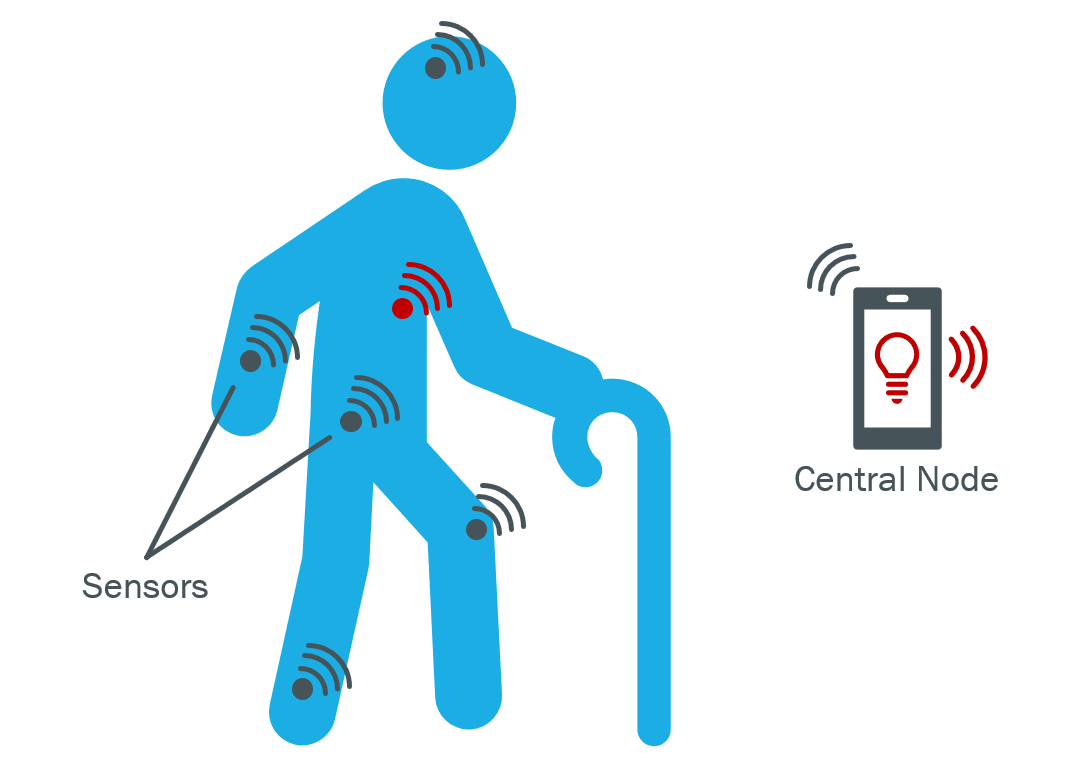
\includegraphics[width=0.4\textwidth, keepaspectratio]{img/BSN-overview.png}
	\caption{Visual representation of the BSN}
	\label{fig:BSN-overview}
\end{figure}

Figure \ref{fig:BSN-overview} depicts the sensors attached to the patient as well as the wireless data transfer to the Central node. In our work, the set sensors comprise a thermometer, an oximeter, a heart rate monitor and an ABP for measuring both the diastolic and systolic artery blood pressure.The patient's health risk can be classified into three levels: low, normal, and high. When a high risk is detected, the Central node signals the individual or a third party about the emergency. The ranges of the sensors were defined by a health expert \cite{pessoa2017building} and their relation with the risk levels are displayed in Table \ref{tab:sensor_ranges}. The patient's health state is considered as \textit{high risk} if at least one of the sensors measurements is in the \textit{high} range. If that is not the case, and one or more resources gauge is within textit{normal} limits, the patient's health state is classified as \textit{normal risk}. Otherwise, the patient's health state is classified as \textit{low risk}.

\begin{table}[!h]
	\centering
	\begin{tabular}{cccccc}
		\hline
		\textbf{Sensor}                  & \textbf{High}                    & \textbf{Moderate}                 & \textbf{Low}                        & \textbf{Moderate}                   & \textbf{High} \\ \hline
		\multicolumn{1}{c|}{Oximeter}    & \multicolumn{1}{c|}{{[}0, 55{]}} & \multicolumn{1}{c|}{(55, 65{]}}   & \multicolumn{1}{c|}{(65, 100{]}}    & \multicolumn{1}{c|}{-}              & -             \\ \hline
		\multicolumn{1}{c|}{Heart Rate}  & \multicolumn{1}{c|}{{[}0, 70{]}} & \multicolumn{1}{c|}{(70, 85{]}}   & \multicolumn{1}{c|}{(85, 97{]}}     & \multicolumn{1}{c|}{(97, 115{]}}    & (115, 300{]}  \\ \hline
		\multicolumn{1}{c|}{Thermometer} & \multicolumn{1}{c|}{{[}0, 35{]}} & \multicolumn{1}{c|}{(35, 36.5{]}} & \multicolumn{1}{c|}{(36.5, 37.5{]}} & \multicolumn{1}{c|}{(37.5, 38.3{]}} & (38.3, 50{]}  \\ \hline
		\multicolumn{1}{c|}{ABPD}        & \multicolumn{1}{c|}{-}           & \multicolumn{1}{c|}{-}            & \multicolumn{1}{c|}{{[}0, 80{]}}    & \multicolumn{1}{c|}{(80, 90{]}}     & (90, 300{]}   \\ \hline
		\multicolumn{1}{c|}{ABPS}        & \multicolumn{1}{c|}{-}           & \multicolumn{1}{c|}{-}            & \multicolumn{1}{c|}{{[}0, 120{]}}   & \multicolumn{1}{c|}{(120, 140{]}}   & (140, 300{]} 
	\end{tabular}
	\label{tab:sensor_ranges}
	\caption{Ranges of the Sensors}
\end{table}

\section{Contextual Goal Model}

Figure \ref{fig:BSN-CGM} shows the Contextual Goal Model (CGM) that represents the Body Sensor Network. This model provides a powerful way of understanding the needs of the stakeholders besides figuring out the motives behind the development of the CPS, by laying out user goals and ways to meet them \cite{ali_goal_based_2010}. The main goal of the BSN \cite{pessoa2017building}, also called root goal, is "G1: Emergency is detected". It is fulfilled by two other goals: "G2: Patient Status is monitored" and "G3: Sampling rate is adjusted". In turn, the goal G2 is achieved when "G4: Vital signs are processed" is achieved. G4 is divided into two other goals: "G5: Vital signs are monitored" and "G6: Vital signs are analyzed". Following the decomposition of the goals, a series of executable tasks are elicited to satisfy them. The context condition \textit{IC} can be set to "low risk", "normal risk" and "high risk" and is utilized in the fulfillment of T3.

\begin{figure}[!h]
	\centering
	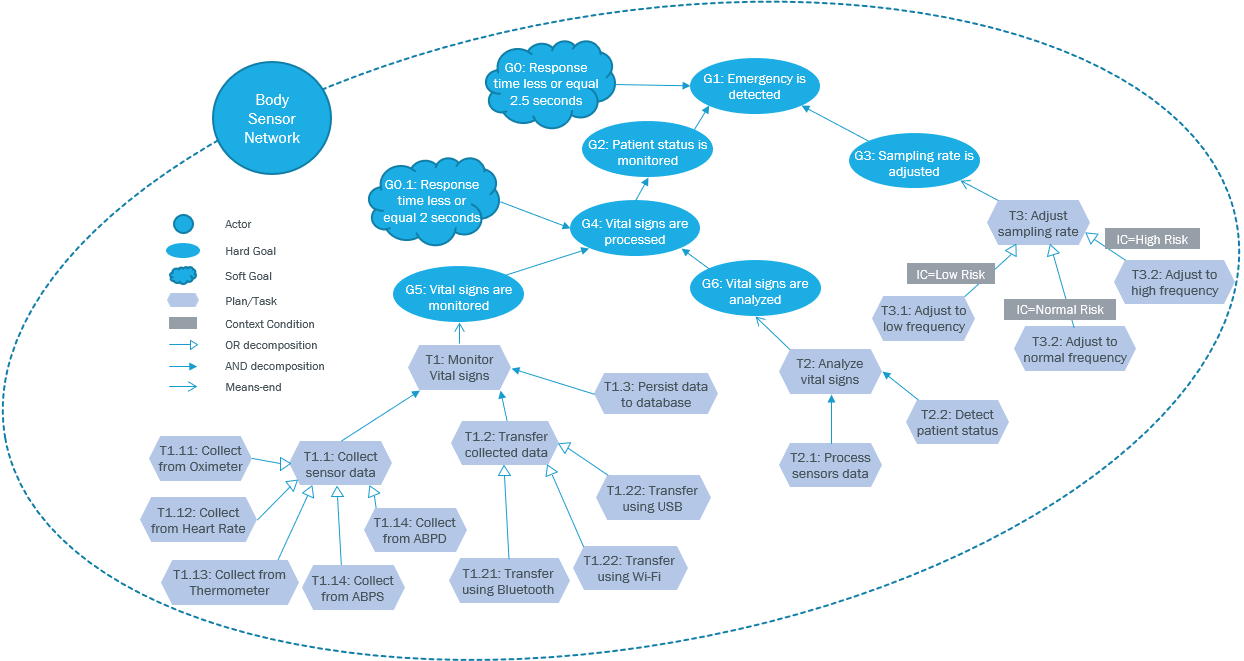
\includegraphics[width=1\textwidth, keepaspectratio]{img/cgm_bsn.png}
	\caption{Contextual Goal Model of the BSN}
	\label{fig:BSN-CGM}
\end{figure}

\section{System Properties}

Another important aspect of the BSN that need to be addressed for the verification process is the definition of the system properties. Rodrigues et al. \cite{seams2018}, by using a CGM for the BSN very similar to the one adopted here, derived a series of properties for the BSN in Timed Computational Tree Logic (TCTL) \cite{henzinger1994symbolic} to verify the satisfiability of the goals modeled through Model Checking. Their work, showed in Table \ref{tab:BSN_TCTL_properties}, bring the sufficient TCTL-like properties to ensure the correct behavior of the CPS by satisfying all the goals specified in the CGM. 

Properties P1 and P2 relate to general aspects of the system behavior by accounting for problems that are common in distributed systems, like deadlocks and the execution of all modules within a cycle, respectively. P3 is related to the root goal and addresses the soft goal G0, which presents a time bound for the execution of a cycle.  P4, P5 and P6 were designed to assess Goal G3 in relation to the context variability that it possess. Property P7, in turn, relates to G2 and was slightly modified here with the addition of the soft goal G0.1. This was done to better clarify some of the processes that are performed during the data processing step of our approach. Besides that, for the verification of the property using an obsever suring the simulation, a time bound needed to be added so that the error state could be reached whithin a cycle. Finally, properties P8, P9 and P10 ensure that the goals G4 and G5 are met and that the data is whithin the expected range.


\begin{table}[!h]
	\begin{tabular}{lccccc}
	\hline
	\textbf{Goal}            & \multicolumn{1}{l}{\textbf{ID}} & \multicolumn{1}{l}{\textbf{Informal Description}}                                                                                                                                                                                                 & \multicolumn{1}{l}{\textbf{Specification in TCTL}} & \textbf{}             & \textbf{} \\ \hline
	\multicolumn{1}{l|}{N/A} & \multicolumn{1}{c|}{P1}         & \multicolumn{1}{l|}{The controlled system is deadlock free.}                                                                                                                                                                                      & \multicolumn{1}{c|}{}                              & \multicolumn{1}{c|}{} &           \\ \hline
	\multicolumn{1}{l|}{N/A} & \multicolumn{1}{c|}{P2}         & \multicolumn{1}{l|}{\makecell{Whenever the scheduler cycle is completed, \\ implies that the central node and the five \\ sensors have been executed}}                                                                                                             & \multicolumn{1}{c|}{}                              & \multicolumn{1}{c|}{} &           \\ \hline
	\multicolumn{1}{c|}{G1}  & \multicolumn{1}{c|}{P3}         & \multicolumn{1}{l|}{Whenever the patients' health} & \multicolumn{1}{c|}{}                              & \multicolumn{1}{c|}{} &           \\ \hline
	\multicolumn{1}{c|}{}    & \multicolumn{1}{c|}{}           & \multicolumn{1}{l|}{}                                                                                                                                                                                                                             & \multicolumn{1}{c|}{}                              & \multicolumn{1}{c|}{} &           \\ \hline
	\multicolumn{1}{c|}{}    & \multicolumn{1}{c|}{}           & \multicolumn{1}{c|}{}                                                                                                                                                                                                                             & \multicolumn{1}{c|}{}                              & \multicolumn{1}{c|}{} &          
	\end{tabular}
	\caption{Major TCTL properties for the verification of the BSN goals \cite{seams2018}}
	\label{tab:BSN_TCTL_properties}
	\end{table}

Moreover, Vogel et al. \cite{vogel2022property} modeled some of the properties defined above as timed-automata observers by using a pattern catalog. Their work intends to use these observers during the Model Checking process, but in our work we will implement them as state machines in the BSN prototype for the verification of the properties during the simulation. The process of creation of the observers based on the properties is thoroughly described in their paper, and referred in Section \ref{sec:property_spec}, whilst the observers that were utilized here can be found in their GitHub repository \cite{2022PSP}.
